% Gabarit pandoc des corrigés publiés (brut et guidé). Contenu sans marque ni nom de site.
% Compilation : lualatex (latexmk -lualatex).
% Le Markdown reste la source unique : ne pas éditer ce fichier .tex à la main.
\documentclass[11pt,a4paper]{article}

% --- Moteur, polices (Latin Modern) et langue ---------------------------------
\usepackage{iftex}
\ifLuaTeX\else\errmessage{Ce document se compile avec lualatex}\fi
\usepackage{amsmath,amssymb,mathtools}
\usepackage{fontspec}
% mathrm=sym : \mathrm prend ses glyphes dans la police mathématique (ℓ, μ, Ω), comme KaTeX.
\usepackage[math-style=TeX,bold-style=TeX,mathrm=sym]{unicode-math}
% Repli pour les glyphes absents de Latin Modern (indices et exposants Unicode,
% flèches, filets des schémas en texte, symboles) : DejaVu, puis Latin Modern Math
% (ℓ, lettres mathématiques Unicode des légendes).
\directlua{
  luaotfload.add_fallback("repliTexte", {"DejaVuSerif:mode=harf;", "DejaVuSans:mode=harf;", "file:latinmodern-math.otf:mode=harf;"})
  luaotfload.add_fallback("repliMono", {"DejaVuSansMono:mode=harf;", "DejaVuSans:mode=harf;", "file:latinmodern-math.otf:mode=harf;"})
}
\setmainfont{Latin Modern Roman}[RawFeature={fallback=repliTexte}]
\setsansfont{Latin Modern Sans}[RawFeature={fallback=repliTexte}]
\setmonofont{Latin Modern Mono}[RawFeature={fallback=repliMono}]
\setmathfont{Latin Modern Math}
\usepackage[french]{babel}
\frenchsetup{SmallCapsFigTabCaptions=false}

% --- Mise en page --------------------------------------------------------------
\usepackage[a4paper,margin=2.2cm,headheight=14pt,footskip=1.2cm]{geometry}
\usepackage{microtype}
\setlength{\emergencystretch}{4em}
\tolerance=1500
\setlength{\parindent}{0pt}
\setlength{\parskip}{0.55\baselineskip plus 2pt minus 1pt}
\usepackage{xcolor}
% Gris nommés : babel-french rend « ! » actif dans le document.
\definecolor{gris2}{gray}{0.98}
\definecolor{gris3}{gray}{0.97}
\definecolor{gris5}{gray}{0.95}
\definecolor{gris35}{gray}{0.65}
\definecolor{gris40}{gray}{0.60}
\definecolor{gris45}{gray}{0.55}
\definecolor{gris50}{gray}{0.50}
\definecolor{gris55}{gray}{0.45}
\definecolor{gris60}{gray}{0.40}
\definecolor{gris65}{gray}{0.35}
\definecolor{gris70}{gray}{0.30}
\definecolor{gris80}{gray}{0.20}
\definecolor{gris85}{gray}{0.15}
\usepackage{graphicx}
\usepackage{float}
\usepackage{caption}
\captionsetup{font=small,labelformat=empty,justification=centering}
\usepackage{booktabs,longtable,array,multirow,calc}
\usepackage{siunitx}
\sisetup{locale=FR}
\usepackage[version=4]{mhchem}
\usepackage{listings}
\usepackage{fancyhdr}
\usepackage{lastpage}
\usepackage[most]{tcolorbox}
\usepackage{enumitem}
\setlist{nosep,leftmargin=*,topsep=2pt}
\usepackage[hidelinks,unicode]{hyperref}
\usepackage{bookmark}
\hypersetup{pdftitle={CCINP MP — Physique-chimie 2026},pdfauthor={Rédigé par IA},pdfcreator={LaTeX},pdfsubject={Corrigé brut}}
\usepackage{xurl}

% --- Pandoc : listes, tableaux, figures ----------------------------------------
\providecommand{\passthrough}[1]{#1}
\providecommand{\tightlist}{\setlength{\itemsep}{0pt}\setlength{\parskip}{0pt}}

\makeatletter
\def\maxwidth{\ifdim\Gin@nat@width>\linewidth\linewidth\else\Gin@nat@width\fi}
\def\maxheight{\ifdim\Gin@nat@height>0.55\textheight 0.55\textheight\else\Gin@nat@height\fi}
\makeatother
\setkeys{Gin}{width=\maxwidth,height=\maxheight,keepaspectratio}
\setcounter{secnumdepth}{-\maxdimen}
\providecommand{\pandocbounded}[1]{#1}
\usepackage{longtable,booktabs,array}

% --- Code (listings) -----------------------------------------------------------
\lstset{
  basicstyle=\ttfamily\small,
  columns=fullflexible,
  keepspaces=true,
  breaklines=true,
  breakatwhitespace=false,
  postbreak=\mbox{\textcolor{gris50}{$\hookrightarrow$}\space},
  frame=single,
  rulecolor=\color{gris35},
  framesep=4pt,
  xleftmargin=5pt,xrightmargin=5pt,
  backgroundcolor=\color{gris3},
  keywordstyle=\bfseries,
  commentstyle=\color{gris65},
  stringstyle=\color{gris80},
  showstringspaces=false,
  tabsize=4,
  extendedchars=true,
  aboveskip=6pt,belowskip=6pt,
}

% --- Macros des corrigés (KaTeX ↔ LaTeX) ---------------------------------------
% Les corrigés sont écrits pour KaTeX : on définit ici ce que KaTeX connaît et
% que LaTeX n'a pas, sans jamais retoucher le Markdown.
\providecommand{\R}{\mathbb{R}}
\providecommand{\N}{\mathbb{N}}
\providecommand{\Z}{\mathbb{Z}}
\providecommand{\Q}{\mathbb{Q}}
\providecommand{\C}{\mathbb{C}}
\providecommand{\dd}{\mathrm{d}}
\providecommand{\llbracket}{\lBrack}
\providecommand{\rrbracket}{\rBrack}
\providecommand{\lBrace}{\lbrace}
\providecommand{\rBrace}{\rbrace}
\providecommand{\Box}{\square}
\providecommand{\Diamond}{\lozenge}
\providecommand{\varnothing}{\emptyset}
\providecommand{\argmax}{\operatorname*{arg\,max}}
\providecommand{\argmin}{\operatorname*{arg\,min}}
\renewcommand{\leq}{\leqslant}
\renewcommand{\geq}{\geqslant}

% Équation hors texte : réduite à la largeur de la ligne si elle déborde.
\newsavebox{\boiteequation}
\newcommand{\equationajustee}[1]{%
  \sbox{\boiteequation}{$\displaystyle #1$}%
  \ifdim\wd\boiteequation>\linewidth
    \[\resizebox{\linewidth}{!}{\usebox{\boiteequation}}\]%
  \else
    \[#1\]%
  \fi}

% --- Encadrés pédagogiques (sobres, lisibles en noir et blanc) -----------------
\tcbset{
  encadre/.style={
    enhanced,breakable,sharp corners,
    colback=white,colframe=gris55,
    boxrule=0.4pt,leftrule=2.2pt,
    left=6pt,right=6pt,top=3pt,bottom=3pt,
    before skip=6pt,after skip=6pt,
    fonttitle=\bfseries\small,coltitle=black,
    attach title to upper,after title={\quad},
    parbox=false,
  }
}
\newtcolorbox{indication}[1]{encadre,colframe=gris45,colback=gris2,title={Indication~#1}}
\newtcolorbox{methode}{encadre,colframe=gris70,title={Méthode}}
\newtcolorbox{piege}{encadre,colframe=gris85,boxrule=0.8pt,leftrule=2.2pt,title={Piège}}
\newtcolorbox{jury}{encadre,colframe=gris60,colback=gris5,title={Jury}}
\newtcolorbox{encadrenote}{encadre,colframe=gris40}

% --- Titres de section ---------------------------------------------------------
\usepackage{titlesec}
\titleformat{\section}{\Large\bfseries}{}{0pt}{}
\titleformat{\subsection}{\large\bfseries}{}{0pt}{}
\titleformat{\subsubsection}{\normalsize\bfseries}{}{0pt}{}
\titlespacing*{\section}{0pt}{14pt plus 4pt minus 2pt}{6pt}
\titlespacing*{\subsection}{0pt}{10pt plus 3pt minus 2pt}{4pt}
\titlespacing*{\subsubsection}{0pt}{8pt plus 2pt minus 2pt}{2pt}

% --- En-tête et pied de page ---------------------------------------------------
\pagestyle{fancy}
\fancyhf{}
\fancyhead[L]{\small\textsc{Corrigé brut} · CCINP MP}
\fancyhead[R]{\small Physique-chimie 2026}
\fancyfoot[L]{\footnotesize Corrigé rédigé par IA, non officiel}
\fancyfoot[R]{\footnotesize \thepage\,/\,\pageref*{LastPage}}
\renewcommand{\headrulewidth}{0.4pt}
\renewcommand{\footrulewidth}{0pt}
\fancypagestyle{plain}{\fancyhf{}\fancyfoot[R]{\footnotesize \thepage\,/\,\pageref*{LastPage}}\fancyfoot[L]{\footnotesize Corrigé rédigé par IA, non officiel}\renewcommand{\headrulewidth}{0pt}}

\begin{document}
\thispagestyle{plain}
\begin{center}
  {\small\scshape Corrigé brut}\par\smallskip
  {\LARGE\bfseries CCINP MP — Physique-chimie 2026\par}\medskip
  {\large CCINP · MP · Physique-chimie · 2026\par}
\end{center}
\vspace{2pt}\hrule\vspace{8pt}

\emph{Corrigé rédigé par IA, non officiel. Signalez toute erreur.}

Épreuve de 4 heures, calculatrices interdites. Les applications numériques sont menées avec la table de logarithmes décimaux de l'annexe et données avec un ou deux chiffres significatifs, comme l'autorise l'énoncé. Base sphérique \((\vec u_r,\vec u_\theta,\vec u_\varphi)\), \(\vec u_z\) unitaire de l'axe des pôles orienté du sud vers le nord.

\hypertarget{partie-i-champ-gravitationnel-et-champ-de-pesanteur}{%
\section{Partie I --- Champ gravitationnel et champ de pesanteur}\label{partie-i-champ-gravitationnel-et-champ-de-pesanteur}}

\hypertarget{q1}{%
\subsection{Q1}\label{q1}}

Une masse ponctuelle \(m\) et une charge ponctuelle \(q\) placées en \(O\) créent en \(M\), repéré par \(\overrightarrow{OM}=r\,\vec u_r\), les champs :

\equationajustee{\vec G(M)=-\frac{Gm}{r^2}\,\vec u_r}

\equationajustee{\vec E(M)=\frac{q}{4\pi\varepsilon_0 r^2}\,\vec u_r}

Le signe \(-\) du champ gravitationnel traduit le caractère toujours attractif de la gravitation. L'identification \(\dfrac{q}{4\pi\varepsilon_0}\leftrightarrow -Gm\) donne les analogies :

\equationajustee{\boxed{\begin{aligned}
q\ &\longleftrightarrow\ m\\
\frac{1}{\varepsilon_0}\ &\longleftrightarrow\ -4\pi G\quad\left(\varepsilon_0\leftrightarrow-\frac{1}{4\pi G}\right)
\end{aligned}}}

Le théorème de Gauss électrostatique s'écrit, pour une surface fermée \(S\) :

\equationajustee{\oint_S\vec E\cdot\mathrm d\vec S_{\rm ext}=\frac{Q_{\rm int}}{\varepsilon_0}}

Il devient : \textbf{le flux du champ gravitationnel sortant d'une surface fermée \(S\) est égal à \(-4\pi G\) fois la masse intérieure, contenue dans le volume \(V\) que \(S\) délimite} :

\equationajustee{\boxed{\oint_{S}\vec G(P)\cdot\mathrm d\vec S_{\rm ext}=-4\pi G\iiint_V\mu(P)\,\mathrm d\tau}}

\hypertarget{q2}{%
\subsection{Q2}\label{q2}}

La boule homogène est invariante par toute rotation autour de \(O\) : la norme du champ ne dépend que de \(r\).

Tout plan contenant \(O\) et \(M\) est plan de symétrie de la distribution de masse. Le champ en \(M\) appartient donc à la droite \((OM)\) :

\equationajustee{\vec G_T(M)=G(r)\,\vec u_r}

On applique le théorème de Gauss à la sphère de centre \(O\) et de rayon \(r\), surface \textbf{fermée} orientée vers l'extérieur. Elle délimite la boule de rayon \(r\), de masse intérieure \(M_{\rm int}(r)\) :

\equationajustee{\begin{aligned}
\oint_S\vec G_T\cdot\mathrm d\vec S_{\rm ext}&=4\pi r^2G(r)\\
&=-4\pi G\,M_{\rm int}(r)
\end{aligned}}

\begin{itemize}
\tightlist
\item
  Pour \(r\ge R_T\), toute la Terre est intérieure : \(M_{\rm int}=M_T=\frac43\pi R_T^3\mu_T\), d'où
  \equationajustee{\boxed{\begin{aligned}\vec G_T(M)&=-\frac{GM_T}{r^2}\,\vec u_r\\&=-\frac{4\pi G\mu_T R_T^3}{3r^2}\,\vec u_r\qquad(r\ge R_T)\end{aligned}}}
\item
  Pour \(r\le R_T\), seule la boule de rayon \(r\) est intérieure : \(M_{\rm int}=\frac43\pi r^3\mu_T\), d'où
  \equationajustee{\boxed{\vec G_T(M)=-\frac{4\pi G\mu_T}{3}\,r\,\vec u_r\ \ (r\le R_T)}}
\end{itemize}

Les deux expressions se raccordent en \(r=R_T\), où la norme vaut \(GM_T/R_T^2\). Le champ est nul au centre.

\hypertarget{q3}{%
\subsection{Q3}\label{q3}}

On applique le principe de superposition. La Terre avec gisement est la somme de deux distributions :

\begin{itemize}
\tightlist
\item
  la Terre homogène pleine, de masse volumique \(\mu_T\) ;
\item
  une boule de centre \(C\) et de rayon \(r'\), de masse volumique \(\mu_p-\mu_T\), qui retire la petite sphère de Terre et la remplace par le pétrole.
\end{itemize}

Cette boule fictive a pour masse :

\equationajustee{m'=\frac43\pi r'^3(\mu_p-\mu_T)<0}

Le point \(M\) lui est extérieur (\(d>r'\)), avec \(\overrightarrow{CM}=d\,\vec u_z\). En \(M\), on a aussi \(\vec u_r=\vec u_z\). D'après Q2, la Terre pleine crée en \(M\), à la surface :

\equationajustee{G_T(M)=-\frac{4\pi G\mu_TR_T}{3}}

La boule fictive crée en \(M\) le champ d'une masse ponctuelle \(m'\) placée en \(C\) :

\equationajustee{\begin{aligned}
\vec G_{\rm corr}(M)&=-\frac{Gm'}{d^2}\,\vec u_z\\
&=\frac{4\pi G r'^3(\mu_T-\mu_p)}{3d^2}\,\vec u_z
\end{aligned}}

Par superposition, \(\vec G_{Tp}=\vec G_T+\vec G_{\rm corr}\) :

\equationajustee{\boxed{G_{Tp}(M)\,\vec u_z=-\frac{4\pi G}{3}\left[\mu_TR_T-\frac{(\mu_T-\mu_p)\,r'^3}{d^2}\right]\vec u_z}}

La variation relative s'en déduit :

\equationajustee{\begin{aligned}
\varepsilon&=\frac{G_T-G_{Tp}}{G_T}\\
&=-\frac{G_{\rm corr}}{G_T}\\
&=\left(1-\frac{\mu_p}{\mu_T}\right)\frac{r'^3}{d^2R_T}
\end{aligned}}

\equationajustee{\boxed{\varepsilon=\left(1-\frac{\mu_p}{\mu_T}\right)\left(\frac{r'}{d}\right)^2\frac{r'}{R_T}}}

Comme \(\mu_p<\mu_T\), le champ correcteur est dirigé vers le haut, opposé au champ terrestre. On a donc \(\varepsilon>0\) et \(|G_{Tp}|<|G_T|\). \textbf{En présence de pétrole, le champ gravitationnel est moins intense} : on a remplacé de la roche par un fluide moins dense.

Application numérique :

\equationajustee{\begin{aligned}
\varepsilon&=\frac56\times\frac14\times\frac{10^{-3}}{4}\\
&=5{,}2\cdot10^{-5}\\
&\approx\boxed{5\cdot10^{-5}}
\end{aligned}}

Cette anomalie est environ \(5\cdot10^{3}\) fois supérieure à la précision relative des gravimètres (\(10^{-8}\)) : \textbf{le gisement est largement détectable}, la gravimétrie est une méthode de prospection pertinente.

\hypertarget{partie-ii-forme-de-la-terre}{%
\section{Partie II --- Forme de la Terre}\label{partie-ii-forme-de-la-terre}}

\hypertarget{q4}{%
\subsection{Q4}\label{q4}}

Le référentiel terrestre \(R'\) est en rotation uniforme, de vecteur \(\vec\Omega=\Omega\vec u_z\), autour de l'axe fixe \(Oz\) du référentiel géocentrique supposé galiléen. Un point \(M\) y subit, outre les forces réelles, deux forces d'inertie :

\begin{itemize}
\tightlist
\item
  la force d'inertie d'entraînement \(\vec F_{ie}=-m\vec a_e\) ; l'entraînement est un mouvement circulaire uniforme de rayon \(HM\), d'accélération centripète \(\vec a_e=-\Omega^2\overrightarrow{HM}\), donc \(\vec F_{ie}=m\Omega^2\overrightarrow{HM}\) ;
\item
  la force de Coriolis \(\vec F_{ic}=-2m\vec\Omega\wedge\vec v_{R'}\).
\end{itemize}

Le poids est défini pour un corps \textbf{au repos} dans \(R'\) : la force de Coriolis est alors nulle. Le poids est la somme de l'attraction gravitationnelle et de la force d'inertie d'entraînement :

\equationajustee{\vec P=m\vec g(M)=m\Big(\underbrace{-\frac{GM_T}{r^2}\vec u_r}_{\text{gravitation}}+\underbrace{\Omega^2\overrightarrow{HM}}_{\text{inertie d'\text{entraînement}}}\Big).}

Ordre de grandeur à la surface : le terme d'entraînement est négligeable (moins de 0,4 \%, cf.~Q6), et

\equationajustee{\begin{aligned}
g&\approx\frac{GM_T}{R_T^2}\\
\log g&=-10{,}17+24{,}78-2\times6{,}81\\
&=0{,}99
\end{aligned}}

d'où \(\boxed{g\approx10\ \mathrm{m\,s^{-2}}}\), soit la valeur bien connue \(9{,}8\ \mathrm{m\,s^{-2}}\).

\hypertarget{q5}{%
\subsection{Q5}\label{q5}}

La force de Coriolis s'écrit \(\vec F_{ic}=-2m\vec\Omega\wedge\vec v\), où \(\vec v\) est la vitesse du train dans \(R'\). La norme d'un produit vectoriel est majorée par le produit des normes : \(\|\vec F_{ic}\|\le2m\Omega v\). Pour \(v=100\ \mathrm{m\,s^{-1}}\) :

\equationajustee{\begin{aligned}
\frac{\|\vec F_{ic}\|}{mg}&\le\frac{2\Omega v}{g}\\
&=\frac{2\times7{,}3\cdot10^{-5}\times100}{9{,}8}\\
&\approx\boxed{1{,}5\cdot10^{-3}}
\end{aligned}}

La force de Coriolis vaut au plus 0,15 \% du poids : elle est négligeable devant lui.

\hypertarget{q6}{%
\subsection{Q6}\label{q6}}

À la surface (\(r=R_T\)), le terme d'inertie d'entraînement a pour norme \(\Omega^2HM=\Omega^2R_T\sin\theta\). Le terme de gravitation a pour norme \(GM_T/R_T^2\). Leur rapport vérifie :

\equationajustee{\begin{aligned}
\frac{\Omega^2R_T\sin\theta}{GM_T/R_T^2}&=\frac{\Omega^2R_T^3}{GM_T}\sin\theta\\
&\le\frac{\Omega^2R_T^3}{GM_T}
\end{aligned}}

\equationajustee{\boxed{\eta=\frac{\Omega^2R_T^3}{GM_T}}}

L'égalité a lieu à l'équateur (\(\theta=\pi/2\)). Le facteur \(R_T^3\) vient de \(R_T\) (distance à l'axe) multiplié par \(R_T^2\) (dénominateur du champ de gravitation). Numériquement :

\equationajustee{\begin{aligned}
\log\eta&=2(-4{,}14)+3(6{,}81)+10{,}17-24{,}78\\
&=-2{,}46
\end{aligned}}

d'où \(\boxed{\eta\approx3{,}5\cdot10^{-3}}\).

Ce rapport est très petit devant 1 : le terme d'inertie d'entraînement est au plus de l'ordre de 0,3 \% du terme gravitationnel, et le champ de pesanteur est très proche du champ de gravitation. Ce petit terme suffit toutefois à rendre \(g\) plus faible à l'équateur et à déformer la Terre (Q8).

\hypertarget{q7}{%
\subsection{Q7}\label{q7}}

\textbf{a)} La force est \(\vec F_G=-\dfrac{GM_Tm}{r^2}\vec u_r\). Pour un déplacement élémentaire \(\mathrm d\vec\ell\), seule sa composante radiale \(\mathrm dr\) travaille :

\equationajustee{\begin{aligned}
\delta W&=\vec F_G\cdot\mathrm d\vec\ell\\
&=-\frac{GM_Tm}{r^2}\,\mathrm dr\\
&=-\mathrm d\!\left(-\frac{GM_Tm}{r}\right)
\end{aligned}}

La force dérive donc de \(-GM_Tm/r+\text{cte}\). Avec \(E_{pG}\to0\) à l'infini, la constante est nulle :

\equationajustee{\boxed{E_{pG}(M)=-\frac{GM_Tm}{r}}}

\textbf{b)} Soit \(\rho=HM\) la distance à l'axe et \(\vec u_\rho\) le vecteur unitaire de \(\overrightarrow{HM}\). La force s'écrit \(\vec F_e=m\Omega^2\rho\,\vec u_\rho\).

Le déplacement \(\mathrm d\vec\ell\) a pour composante \(\mathrm d\rho\) selon \(\vec u_\rho\) ; ses autres composantes sont orthogonales à \(\vec F_e\). Ainsi :

\equationajustee{\begin{aligned}
\delta W&=m\Omega^2\rho\,\mathrm d\rho\\
&=-\mathrm d\!\left(-\tfrac12m\Omega^2\rho^2\right)
\end{aligned}}

La force dérive donc de \(E_{pe}=-\frac12m\Omega^2\rho^2+\text{cte}\). La constante est nulle avec \(E_{pe}=0\) en \(r=0\), où \(\rho=0\). Comme \(\rho=r\sin\theta\) :

\equationajustee{\boxed{\begin{aligned}E_{pe}(M)&=-\frac12m\Omega^2\left(\overrightarrow{HM}\right)^2\\&=-\frac12m\Omega^2r^2\sin^2\theta\end{aligned}}}

\textbf{c)} Le poids est la somme des deux forces, qui dérivent chacune d'une énergie potentielle : les énergies potentielles s'ajoutent.

\equationajustee{\boxed{E_{pp}(M)=-\frac{GM_Tm}{r}-\frac12m\Omega^2r^2\sin^2\theta}}

\hypertarget{q8}{%
\subsection{Q8}\label{q8}}

Au pôle Nord, \(\theta=0\) et \(E_{pp}(N)=-GM_Tm/r_n\). La trace de \((\Sigma)\) dans un plan méridien vérifie \(E_{pp}(M)=E_{pp}(N)\), soit, après division par \(-m\) :

\equationajustee{\begin{aligned}
\frac{GM_T}{r}+\frac12\Omega^2r^2\sin^2\theta&=\frac{GM_T}{r_n}\\
\frac1r&=\frac1{r_n}-\frac{\Omega^2r^2\sin^2\theta}{2GM_T}\\
r&=\frac{r_n}{1-\dfrac{\Omega^2r_nr^2\sin^2\theta}{2GM_T}}
\end{aligned}}

Le terme soustrait au dénominateur est au plus de l'ordre de \(\Omega^2R_T^3/(2GM_T)=\eta/2\approx2\cdot10^{-3}\ll1\), car \(r\) et \(r_n\) restent voisins de \(R_T\).

Au premier ordre en ce petit terme, \((1-u)^{-1}\approx1+u\). Dans le terme correctif, on peut remplacer \(r\) par \(r_n\) : l'erreur commise est du second ordre. D'où :

\equationajustee{\boxed{\begin{aligned}
r(\theta)&\approx r_n\left(1+\varepsilon\sin^2\theta\right)\\
\varepsilon&=\frac{\Omega^2r_n^3}{2GM_T}\\
&=\frac{\eta}{2}\left(\frac{r_n}{R_T}\right)^3
\end{aligned}}}

Allure (figure 1) : \(r\) est minimal aux pôles, où \(r=r_n\), et maximal à l'équateur, où \(r=r_n(1+\varepsilon)\). Au premier ordre, la trace est une ellipse aplatie aux pôles.

\begin{figure}[H]
\centering
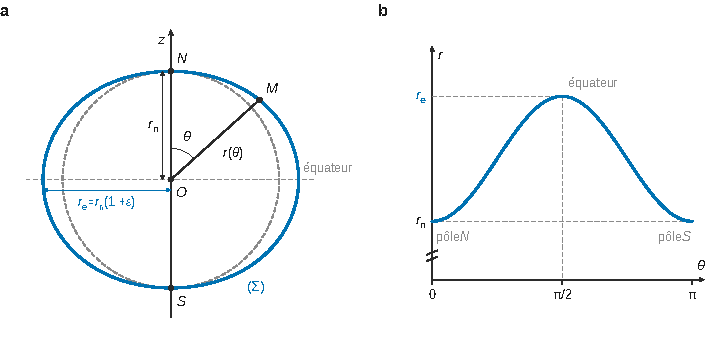
\includegraphics{figures/q8-equipotentielle.pdf}
\caption*{Figure 1 --- équipotentielle (Σ) dans un plan méridien, aplatissement
exagéré, et allure de r(θ) pour 0 ≤ θ ≤ π}
\end{figure}

Aplatissement, avec \(r_e=r(\pi/2)\) et \(r_n\approx R_T\) :

\equationajustee{\begin{aligned}
\varepsilon'&=\frac{r_e-r_n}{r_n}\\
&=\varepsilon\\
&=\frac{\eta}{2}\left(\frac{r_n}{R_T}\right)^3
\end{aligned}}

\equationajustee{\boxed{\varepsilon'\approx\frac{\eta}{2}\approx1{,}7\cdot10^{-3}\approx\frac1{580}}}

(L'aplatissement réel, \(1/298\), est environ double : le modèle néglige la déformation du champ gravitationnel lui-même.)

\hypertarget{partie-iii-duxe9termination-optique-du-champ-de-pesanteur}{%
\section{Partie III --- Détermination optique du champ de pesanteur}\label{partie-iii-duxe9termination-optique-du-champ-de-pesanteur}}

\hypertarget{q9}{%
\subsection{Q9}\label{q9}}

\textbf{a)} En négligeant le terme d'entraînement, \(g(h)=GM_T/(R_T+h)^2\). Comme \(h/R_T\approx1{,}6\cdot10^{-7}\ll1\), un développement limité au premier ordre, \((1+u)^{-2}\approx1-2u\), donne :

\equationajustee{\begin{aligned}
\frac{g(h)-g(0)}{g(0)}&=\left(1+\frac h{R_T}\right)^{-2}-1\\
&\approx-\frac{2h}{R_T}\\
&=-\frac{2}{6{,}4\cdot10^6}\\
&\approx\boxed{-3\cdot10^{-7}}
\end{aligned}}

Sur 1 m de chute, \(g\) varie de quelques \(10^{-7}\) en valeur relative : on peut le considérer constant.

\textbf{b)} L'axe vertical est orienté vers le bas, d'origine \(O_{1,0}\), position de \(O_1\) à \(t=0\). Dans le vide, seul le poids agit, et il est dirigé dans le sens positif de l'axe. Le principe fondamental de la dynamique donne \(\ddot z_1=+g\), avec \(z_1(0)=0\) et \(\dot z_1(0)=0\) :

\equationajustee{\boxed{z_1(t)=\frac12gt^2}}

\hypertarget{q10}{%
\subsection{Q10}\label{q10}}

\textbf{a)} Dans l'air (\(n=1\)), chemin optique et longueur géométrique coïncident. On suit les rayons sur la figure 3(a) avec les lois de la réflexion sur les séparatrices et le miroir inclinés à 45°, et la propriété du coin de cube, qui renvoie la lumière parallèlement à elle-même :

\begin{itemize}
\tightlist
\item
  rayon (1) : transmis par \(S_{p1}\), il va de \(O\) à \(J\), où \(S_{p3}\) le réfléchit vers \(P\) ;
\item
  rayon (2) : réfléchi vers le haut par \(S_{p1}\), il est renvoyé vers le bas par le coin de cube \(C_1\) ;
\item
  il traverse ensuite \(S_{p1}\) puis \(S_{p2}\) et descend jusqu'au coin de cube fixe \(C_2\), qui le renvoie vers le haut ;
\item
  en \(K\), \(S_{p2}\) le réfléchit vers \(H\), et le miroir \(M\) le renvoie vers le haut ;
\item
  il traverse enfin \(S_{p3}\) en \(J\) et atteint \(P\) (figure 2).
\end{itemize}

\begin{figure}[H]
\centering
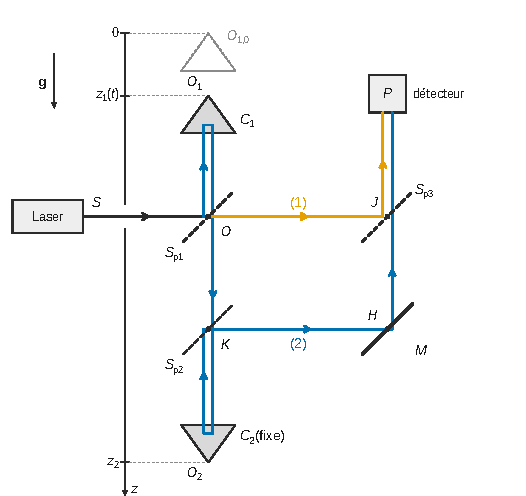
\includegraphics{figures/q10-trajets-mach-zehnder.pdf}
\caption*{Figure 2 --- trajets des rayons (1) et (2) dans l'interféromètre de la
figure 3(a), axe z descendant d'origine O₁,₀}
\end{figure}

On repère les points par des cotes \(Z\) ascendantes et on note \(L=OJ=KH\). Les chemins optiques sont :

\equationajustee{\begin{aligned}
(2)&=2(Z_{O_1}-Z_O)+(Z_O-Z_K)+2(Z_K-Z_{O_2})+L+(Z_J-Z_H)+JP\\
(1)&=L+JP
\end{aligned}}

Comme \(Z_J-Z_H=Z_O-Z_K\), toutes les longueurs fixes se compensent :

\equationajustee{\begin{aligned}
\delta&=(2)-(1)\\
&=2(Z_{O_1}-Z_{O_2})
\end{aligned}}

Sur l'axe descendant d'origine \(O_{1,0}\), on a \(Z_{O_1}-Z_{O_2}=z_2-z_1(t)\), d'où :

\equationajustee{\boxed{\begin{aligned}\delta(P,t)&=2\big(z_2-z_1(t)\big)\\&=2z_2-gt^2\end{aligned}}}

\textbf{b)} Les deux ondes sont issues du même laser par division d'amplitude : elles sont cohérentes. Pour deux ondes de même intensité \(I_0\), la formule de Fresnel donne :

\equationajustee{I=2I_0\left[1+\cos\left(\frac{2\pi\delta}{\lambda}\right)\right]}

On introduit l'ordre d'interférence \(p(t)=\delta(P,t)/\lambda\). L'intensité est minimale (nulle) quand \(\cos(2\pi p)=-1\), c'est-à-dire pour un ordre demi-entier :

\equationajustee{p=k+\frac12,\qquad k\in\mathbb Z}

Comme \(\delta\) décroît strictement avec \(t\), l'ordre décroît aussi. Deux minima successifs ont des ordres qui diffèrent d'exactement 1 : entre \(t_0\) et \(t_q\), l'ordre a diminué de \(q\). D'une part :

\equationajustee{\boxed{\Delta_q=\delta(P,t_q)-\delta(P,t_0)=-q\lambda}}

D'autre part, avec \(\delta=2z_2-gt^2\) :

\equationajustee{\Delta_q=-g\left(t_q^2-t_0^2\right)}

En égalant les deux expressions :

\equationajustee{\boxed{g=\frac{q\lambda}{t_q^2-t_0^2}}}

\textbf{c)} On pose \(y(q)=t_q^2-t_0^2\). D'après (b), cette fonction est linéaire en \(q\) :

\equationajustee{y(q)=\frac{\lambda}{g}\,q}

On relève sur la figure 3(b) les instants \(t_q\) des minima successifs, on trace \(y\) en fonction de \(q\) et on ajuste une droite passant par l'origine. Sa pente vaut \(a=\lambda/g\).

Les temps étant lus en microsecondes, la pente mesurée est \(a=64\,598\ \mu\mathrm s^2=6{,}4598\cdot10^{-8}\ \mathrm s^2\). Alors :

\equationajustee{\begin{aligned}
g&=\frac{\lambda}{a}\\
&=\frac{632{,}82\cdot10^{-9}\ \mathrm m}{64\,598\cdot10^{-12}\ \mathrm s^2}\\
&\approx\boxed{9{,}796\ \mathrm{m\,s^{-2}}}
\end{aligned}}

ce qui redonne \(g=9{,}7961\ \mathrm{m\,s^{-2}}\) à l'arrondi de la pente près.

\hypertarget{partie-iv-le-calcaire-et-largile-des-richesses-du-sol-bon-marchuxe9}{%
\section{Partie IV --- Le calcaire et l'argile : des richesses du sol bon marché}\label{partie-iv-le-calcaire-et-largile-des-richesses-du-sol-bon-marchuxe9}}

\hypertarget{partie-iv.1-calcination-du-calcaire}{%
\subsection{Partie IV.1 --- Calcination du calcaire}\label{partie-iv.1-calcination-du-calcaire}}

\hypertarget{q11}{%
\subsection{Q11}\label{q11}}

\textbf{a)} Dans l'approximation d'Ellingham, \(\Delta_rH_1^0\) et \(\Delta_rS_1^0\) ne dépendent pas de \(T\), et :

\equationajustee{\Delta_rG_1^0=\Delta_rH_1^0-T\Delta_rS_1^0}

Par identification avec l'expression donnée :

\equationajustee{\boxed{\Delta_rH_1^0=177{,}4\ \mathrm{kJ\,mol^{-1}}>0}}

\textbf{La réaction est endothermique.}

\textbf{b)} L'identification donne aussi :

\equationajustee{\boxed{\begin{aligned}\Delta_rS_1^0&=+0{,}1589\ \mathrm{kJ\,K^{-1}\,mol^{-1}}\\&=159\ \mathrm{J\,K^{-1}\,mol^{-1}}\end{aligned}}}

Ce signe positif est attendu : la réaction produit une mole de gaz à partir d'un solide (\(\Delta\nu_{\rm gaz}=+1\)), le désordre augmente.

\textbf{c)} La relation \(\Delta_rG_1^0=-RT\ln K_1^0\) donne, avec \(\Delta_rG_1^0\) en \(\mathrm{J\,mol^{-1}}\) :

\equationajustee{\boxed{\begin{aligned}K_1^0(T)&=\exp\!\left(-\frac{177\,400-158{,}9\,T}{RT}\right)\\&=\exp\!\left(19{,}1-\frac{2{,}13\cdot10^4}{T}\right)\end{aligned}}}

On a \(K_1^0=1\) si et seulement si \(\Delta_rG_1^0=0\) :

\equationajustee{\boxed{\begin{aligned}T_{1,i}&=\frac{177{,}4}{0{,}1589}\\&=1116\ \mathrm K\ \ (843\ ^\circ\mathrm C)\end{aligned}}}

\textbf{d)} Les solides, purs et seuls dans leur phase, ont une activité égale à 1 ; le gaz, supposé parfait, a pour activité \(P_{\mathrm{CO_2}}/P^0\) :

\equationajustee{\boxed{Q_{r,1}=\frac{a(\mathrm{CaO})\,a(\mathrm{CO_2})}{a(\mathrm{CaCO_3})}=\frac{P_{\mathrm{CO_2}}}{P^0}}}

\hypertarget{q12}{%
\subsection{Q12}\label{q12}}

\textbf{a)} De même, \(\Delta_rH_2^0=118{,}0\ \mathrm{kJ\,mol^{-1}}\) et \(\Delta_rS_2^0=175\ \mathrm{J\,K^{-1}\,mol^{-1}}\). La température d'inversion est \(T_{2,i}=674\ \mathrm K\) (401 °C).

Pour chaque réaction \(k\), \(\Delta_rG_k=\Delta_rG_k^0+RT\ln Q_{r,k}\). Sous \(P_{\mathrm{CO_2}}=P^0\), les deux quotients valent 1, donc \(\Delta_rG_k=\Delta_rG_k^0\). En chauffant :

\begin{itemize}
\tightlist
\item
  pour \(T<674\) K, \(\Delta_rG_1^0>0\) et \(\Delta_rG_2^0>0\) : aucune décomposition ;
\item
  à \(T=674\) K, l'équilibre (2) s'établit ; tant qu'on apporte de la chaleur, \(\mathrm{MgCO_3}\) se décompose à température constante, jusqu'à disparition totale ;
\item
  au-delà, \(\Delta_rG_2<0\) et il n'y a plus de réactif : rupture d'équilibre (2) ;
\item
  de 674 K à 1116 K, le solide contient \(\mathrm{CaCO_3}\) et \(\mathrm{MgO}\) ;
\item
  à \(T=1116\) K, \(\mathrm{CaCO_3}\) se décompose à son tour, totalement, à température constante.
\end{itemize}

\textbf{Les deux équilibres ne peuvent pas être simultanés.} La phase gazeuse est commune aux deux équilibres. Leur coexistence imposerait les deux relations \(P_{\mathrm{CO_2}}=K_1^0P^0\) et \(P_{\mathrm{CO_2}}=K_2^0P^0\), donc \(K_1^0(T)=K_2^0(T)\), soit \(\Delta_rG_1^0(T)=\Delta_rG_2^0(T)\) :

\equationajustee{\begin{aligned}
177{,}4-0{,}1589\,T&=118{,}0-0{,}175\,T\\
T&=-\frac{59{,}4}{0{,}0161}\\
&\approx-3{,}7\cdot10^3\ \mathrm K
\end{aligned}}

Cette température négative est impossible. Sous \(P^0\), les décompositions sont donc successives ; \(\mathrm{MgCO_3}\), moins stable, se décompose en premier.

\textbf{b)} On raisonne sur 100 g de mélange contenant \(x\) g de \(\mathrm{MgCO_3}\), de masse molaire \(24+12+48=84\ \mathrm{g\,mol^{-1}}\). La première perte de masse est le \(\mathrm{CO_2}\) (\(44\ \mathrm{g\,mol^{-1}}\)) libéré par la décomposition totale de \(\mathrm{MgCO_3}\) ; une mole de carbonate libère une mole de gaz :

\equationajustee{\begin{aligned}
\frac{44\,x}{84}&=2{,}2\\
x&=\frac{2{,}2\times84}{44}\\
&=\boxed{4{,}2\ \%}
\end{aligned}}

Cette teneur est inférieure à la limite de 6 \% : le calcaire convient. La seconde perte de masse, due à \(\mathrm{CaCO_3}\) (\(100\ \mathrm{g\,mol^{-1}}\)), vaut \(0{,}44\times95{,}8\approx42\) g pour 100 g de mélange initial.

\hypertarget{partie-iv.2-obtention-dun-ciment}{%
\subsection{Partie IV.2 --- Obtention d'un ciment}\label{partie-iv.2-obtention-dun-ciment}}

\hypertarget{q13}{%
\subsection{Q13}\label{q13}}

\equationajustee{\begin{aligned}
\text{A :}\quad & 3\,\mathrm{CaO_{(s)}}+\mathrm{SiO_{2(s)}}\longrightarrow\mathrm{Ca_3SiO_{5(s)}}\\
\text{B :}\quad & 2\,\mathrm{CaO_{(s)}}+\mathrm{SiO_{2(s)}}\longrightarrow\mathrm{Ca_2SiO_{4(s)}}\\
\text{C :}\quad & 3\,\mathrm{CaO_{(s)}}+\mathrm{Al_2O_{3(s)}}\longrightarrow\mathrm{Ca_3Al_2O_{6(s)}}\\
\text{D :}\quad & 4\,\mathrm{CaO_{(s)}}+\mathrm{Al_2O_{3(s)}}+\mathrm{Fe_2O_{3(s)}}\longrightarrow\mathrm{Ca_4Al_2Fe_2O_{10(s)}}
\end{aligned}}

Bilans en oxygène : 5, 4, 6 et 10 atomes de part et d'autre.

\hypertarget{q14}{%
\subsection{Q14}\label{q14}}

On raisonne sur 100 g de ciment. Le composant \(j\) (\(j=5,\dots,8\)) y a une masse \(p_j\) (en g), soit une quantité de matière \(p_j/M_j\).

Une mole du composant \(j\) contient \(\nu_{ij}\) moles de l'oxyde \(i\) (\(i=1,\dots,4\)), lues sur les formules oxydes du tableau 2. La masse d'oxyde \(i\) apportée par le composant \(j\) vaut donc :

\equationajustee{m_{ij}=\nu_{ij}\,\frac{M_i}{M_j}\,p_j}

Les hypothèses (H1) à (H4) garantissent que chaque oxyde du mélange réactionnel se retrouve entièrement dans les composants indiqués ; 100 g de mélange donnent 100 g de ciment. En sommant sur \(j\), \(p_i=\sum_j\beta_{ij}p_j\), avec :

\equationajustee{\boxed{\beta_{ij}=\nu_{ij}\,\frac{M_i}{M_j}}}

\equationajustee{\begin{aligned}
p_1&=3\tfrac{M_1}{M_5}p_5+2\tfrac{M_1}{M_6}p_6+3\tfrac{M_1}{M_7}p_7+4\tfrac{M_1}{M_8}p_8\\
p_2&=\tfrac{M_2}{M_5}p_5+\tfrac{M_2}{M_6}p_6\\
p_3&=\tfrac{M_3}{M_7}p_7+\tfrac{M_3}{M_8}p_8\\
p_4&=\tfrac{M_4}{M_8}p_8
\end{aligned}}

Ligne 5 du script :

\begin{lstlisting}[language=Python]
gob=np.array([[3*M1/M5, 2*M1/M6, 3*M1/M7, 4*M1/M8],
              [  M2/M5,   M2/M6,       0,       0],
              [      0,       0,   M3/M7,   M3/M8],
              [      0,       0,       0,   M4/M8]])
\end{lstlisting}

Avec \texttt{oxy=\allowbreak{}{[}62,\allowbreak{}\ 24,\allowbreak{}\ 9,\allowbreak{}\ 5{]}\allowbreak{}}, le script affiche \texttt{cim=\allowbreak{}\ {[}\ 2.51\ 66.91\ 15.33\ 15.25{]}\allowbreak{}}, de somme 100 (conservation de la masse) : environ 2,5 \% de A, 66,9 \% de B, 15,3 \% de C et 15,3 \% de D.

La matrice est inversible. La dernière ligne donne \(p_8\), la troisième \(p_7\) ; il reste un système \(2\times2\) en \((p_5,p_6)\) dont le déterminant vaut \(M_1M_2/(M_5M_6)\neq0\).

Remarque : le script pose \texttt{M4=159} alors que le tableau 1 donne \(160\ \mathrm{g\,mol^{-1}}\) (d'où \(M_8=485\) au lieu de 486) ; l'écart est sans conséquence (\(0{,}05\) point au plus sur les pourcentages).

\hypertarget{q15}{%
\subsection{Q15}\label{q15}}

Une masse \(m_c\) de ciment contient la masse \(m_cp_j/100\) du composant \(j\), soit la quantité de matière \(n_j=m_cp_j/(100M_j)\).

Chaque mole de A, B, C et D fixe respectivement 3, 2, 6 et 10 moles d'eau. La quantité d'eau consommée est donc :

\equationajustee{n_e=3n_5+2n_6+6n_7+10n_8}

Sa masse est \(m_e=M_0n_e\). En divisant par \(m_c\) :

\equationajustee{\boxed{r=\frac{m_e}{m_c}=\frac{M_0}{100}\left(\frac{3p_5}{M_5}+\frac{2p_6}{M_6}+\frac{6p_7}{M_7}+\frac{10p_8}{M_8}\right)}}

Le facteur 100 vient de \(p_5+p_6+p_7+p_8=100\) : les \(p_j\) sont des pourcentages. Le rapport est bien sans dimension. Avec les valeurs de Q14 et \(M_0=18\ \mathrm{g\,mol^{-1}}\), on trouve \(r\approx0{,}26\).

\hypertarget{q16}{%
\subsection{Q16}\label{q16}}

\textbf{a)} Le produit de solubilité \(K_s\) est la constante de l'équilibre de dissolution du solide. Cet équilibre est réalisé quand la solution est saturée, c'est-à-dire en présence du solide :

\equationajustee{\mathrm{Ca(OH)_{2(s)}}=\mathrm{Ca^{2+}_{(aq)}}+2\,\mathrm{OH^-_{(aq)}}}

\equationajustee{K_s=\frac{[\mathrm{Ca^{2+}}][\mathrm{OH^-}]^2}{(c^0)^3}}

La solubilité \(s\) est la quantité maximale de solide que l'on peut dissoudre par litre de solution. Dans la solution saturée, \([\mathrm{Ca^{2+}}]=s\) et \([\mathrm{OH^-}]=2s\), l'autoprotolyse de l'eau étant négligeable. Donc \(K_s=4s^3\) (concentrations en \(\mathrm{mol\,L^{-1}}\)) :

\equationajustee{\begin{aligned}
s&=\left(\frac{K_s}{4}\right)^{1/3}\\
\log s&=\frac{-5{,}2-0{,}60}{3}\\
&=-1{,}93\\
[\mathrm{OH^-}]&=2s\\
&\approx2{,}3\cdot10^{-2}\ \mathrm{mol\,L^{-1}}
\end{aligned}}

\equationajustee{\begin{aligned}
\mathrm{pH}&=14+\log(2s)\\
&\approx\boxed{12{,}4}
\end{aligned}}

\textbf{b)} En milieu basique, le fer(III) précipite : il est sous forme d'hydroxyde solide, et non d'ions \(\mathrm{Fe^{3+}}\). Les demi-équations sont :

\equationajustee{\mathrm{Fe_{(s)}}+3\,\mathrm{OH^-}=\mathrm{Fe(OH)_{3(s)}}+3e^-}

\equationajustee{\mathrm{O_2}+2\,\mathrm{H_2O}+4e^-=4\,\mathrm{OH^-}}

\equationajustee{\boxed{4\,\mathrm{Fe_{(s)}}+3\,\mathrm{O_{2}}+6\,\mathrm{H_2O}\longrightarrow4\,\mathrm{Fe(OH)_{3(s)}}}}

\textbf{Passivation} : le métal oxydé se recouvre d'une couche compacte, adhérente et très peu soluble d'oxyde ou d'hydroxyde qui l'isole du milieu ; la corrosion devient alors extrêmement lente. Sur la courbe courant-potentiel, le courant anodique chute à une valeur résiduelle très faible sur un domaine de potentiel. À pH 12,4, le fer des armatures est passivé : le béton protège l'acier.

\textbf{c)} En milieu acide, le fer(III) est soluble : l'oxydation donne des ions et non une couche protectrice.

\equationajustee{4\,\mathrm{Fe_{(s)}}+3\,\mathrm{O_2}+12\,\mathrm{H^+}\longrightarrow4\,\mathrm{Fe^{3+}}+6\,\mathrm{H_2O}}

Les ions \(\mathrm{H^+}\) attaquent aussi le fer :

\equationajustee{\mathrm{Fe_{(s)}}+2\,\mathrm{H^+}\longrightarrow\mathrm{Fe^{2+}}+\mathrm{H_{2(g)}}}

Une couche d'hydroxyde éventuellement formée se dissout (\(\mathrm{Fe(OH)_3}+3\,\mathrm{H^+}\to\mathrm{Fe^{3+}}+3\,\mathrm{H_2O}\)). \textbf{Il n'y a plus de passivation : le fer se corrode.} C'est ce qui menace le béton armé lorsque son milieu interstitiel s'acidifie (carbonatation, pluies acides) : la rouille, plus volumineuse que le fer, fait éclater le béton et expose de nouvelles armatures.

\hypertarget{q17}{%
\subsection{Q17}\label{q17}}

La masse molaire de K est \(M_K=102+60x+18y\) (en \(\mathrm{g\,mol^{-1}}\)). Une mole de K contient \(y\) moles d'eau et \(x\) moles de silice.

La perte de masse à 550 °C est le départ de l'eau de constitution : c'est la fraction massique d'eau dans K. La seconde donnée est la fraction massique de silice :

\equationajustee{\boxed{\left\{\begin{aligned}\frac{18\,y}{102+60x+18y}&=0{,}140\\[1mm]\frac{60\,x}{102+60x+18y}&=0{,}465\end{aligned}\right.}}

(Sa résolution, non demandée, donne \(x=y=2\) : kaolinite \(\mathrm{Al_2O_3\cdot2SiO_2\cdot2H_2O}\).)

\hypertarget{partie-iv.3-les-pluies-acides}{%
\subsection{Partie IV.3 --- Les pluies acides}\label{partie-iv.3-les-pluies-acides}}

\hypertarget{q18}{%
\subsection{Q18}\label{q18}}

\textbf{a)} Première acidité :

\equationajustee{\mathrm{H_2CO_3}+\mathrm{H_2O}=\mathrm{HCO_3^-}+\mathrm{H_3O^+}}

\equationajustee{Q_{r,1}=\frac{[\mathrm{HCO_3^-}][\mathrm{H_3O^+}]}{[\mathrm{H_2CO_3}]\,c^0}}

Seconde acidité :

\equationajustee{\mathrm{HCO_3^-}+\mathrm{H_2O}=\mathrm{CO_3^{2-}}+\mathrm{H_3O^+}}

\equationajustee{Q_{r,2}=\frac{[\mathrm{CO_3^{2-}}][\mathrm{H_3O^+}]}{[\mathrm{HCO_3^-}]\,c^0}}

avec \(c^0=1\ \mathrm{mol\,L^{-1}}\) et \(a(\mathrm{H_2O})=1\) (solvant). À l'équilibre, \(Q_{r,1}=K_{a1}\) et \(Q_{r,2}=K_{a2}\).

\textbf{b)} La forme la plus protonée prédomine aux faibles pH, la plus déprotonée aux pH élevés, l'ampholyte entre les deux :

\equationajustee{\boxed{\begin{aligned}(1)&=\mathrm{H_2CO_3}\ (\mathrm{CO_{2,aq},H_2O})\\(2)&=\mathrm{HCO_3^-}\\(3)&=\mathrm{CO_3^{2-}}\end{aligned}}}

\textbf{c)} D'après la loi d'action des masses :

\equationajustee{\mathrm{pH}=\mathrm pK_{a1}+\log\frac{[\mathrm{HCO_3^-}]}{[\mathrm{H_2CO_3}]}}

À l'intersection de deux courbes conjuguées (50 \% chacune), \(\mathrm{pH}=\mathrm pK_a\). On lit \(\mathrm{pH}\approx6{,}3\) pour (1)/(2) et \(\mathrm{pH}\approx10{,}3\) pour (2)/(3). Avec \(K_a=10^{-\mathrm pK_a}\) :

\equationajustee{\boxed{\begin{aligned}K_{a1}&=10^{-6{,}3}\approx5\cdot10^{-7}\\K_{a2}&=10^{-10{,}3}\approx5\cdot10^{-11}\end{aligned}}}

(Contrôle : le maximum de la courbe (2) est à \(\mathrm{pH}=(6{,}3+10{,}3)/2=8{,}3\).)

\hypertarget{q19}{%
\subsection{Q19}\label{q19}}

L'équilibre \(\mathrm{CO_{2(g)}}+\mathrm{H_2O}=(\mathrm{CO_{2(aq)}},\allowbreak \mathrm{H_2O})\) est réalisé en présence de l'atmosphère, réservoir de \(\mathrm{CO_2}\) de composition fixée. Avec \(P_{\mathrm{CO_2}}=x_{\mathrm{CO_2}}P\) :

\equationajustee{\begin{aligned}
K^0&=\frac{c/c^0}{P_{\mathrm{CO_2}}/P^0}\\
c&=K^0(T)\,x_{\mathrm{CO_2}}\,\frac{P}{P^0}\,c^0
\end{aligned}}

À température et pression fixées, tous les termes du second membre sont fixés : \textbf{\(c\) est constante}, quelles que soient les réactions acido-basiques en solution (le gaz renouvelle le \(\mathrm{CO_2}\) dissous consommé). Pour \(P=P^0\) :

\equationajustee{\begin{aligned}
c&=3{,}1\cdot10^{-2}\times3{,}4\cdot10^{-4}\\
&=1{,}1\cdot10^{-5}\ \mathrm{mol\,L^{-1}}
\end{aligned}}

Électroneutralité, avec \(h=[\mathrm{H_3O^+}]\) :

\equationajustee{h=[\mathrm{HCO_3^-}]+2[\mathrm{CO_3^{2-}}]+[\mathrm{OH^-}]}

La solution est acide, donc \([\mathrm{OH^-}]\ll h\) ; la seconde acidité est négligeable, à vérifier. Alors \(h\approx[\mathrm{HCO_3^-}]\) et \(K_{a1}=h^2/c\) :

\equationajustee{\begin{aligned}
\mathrm{pH}&=\frac12\left(\mathrm pK_{a1}-\log c\right)\\
&=\frac12(6{,}3+4{,}98)\\
&\approx\boxed{5{,}6}
\end{aligned}}

Concentrations (en \(\mathrm{mol\,L^{-1}}\)) :

\begin{longtable}[]{@{}
  >{\raggedright\arraybackslash}p{(\columnwidth - 2\tabcolsep) * \real{0.4688}}
  >{\raggedright\arraybackslash}p{(\columnwidth - 2\tabcolsep) * \real{0.5012}}@{}}
\toprule\noalign{}
\begin{minipage}[b]{\linewidth}\raggedright
Espèce
\end{minipage} & \begin{minipage}[b]{\linewidth}\raggedright
Concentration
\end{minipage} \\
\midrule\noalign{}
\endhead
\bottomrule\noalign{}
\endlastfoot
\(\mathrm{H_2CO_3}\) (soit \(\mathrm{CO_{2,aq}}\)) & \(c=1{,}1\cdot10^{-5}\) \\
\(\mathrm{H_3O^+}\) & \(h=\sqrt{K_{a1}c}=2{,}3\cdot10^{-6}\) \\
\(\mathrm{HCO_3^-}\) & \(\approx h=2{,}3\cdot10^{-6}\) \\
\(\mathrm{OH^-}\) & \(K_e/h=4{,}3\cdot10^{-9}\) \\
\(\mathrm{CO_3^{2-}}\) & \(K_{a2}[\mathrm{HCO_3^-}]/h=K_{a2}=5\cdot10^{-11}\) \\
\end{longtable}

Vérification : \([\mathrm{OH^-}]\) et \(2[\mathrm{CO_3^{2-}}]\) sont négligeables devant \(h\). Une eau de pluie en équilibre avec l'air est naturellement acide (pH 5,6). L'augmentation de \(x_{\mathrm{CO_2}}\), dont la production de ciment est une source importante, l'acidifie davantage.

\hypertarget{partie-v-quelques-propriuxe9tuxe9s-thermodynamiques-de-la-terre}{%
\section{Partie V --- Quelques propriétés thermodynamiques de la Terre}\label{partie-v-quelques-propriuxe9tuxe9s-thermodynamiques-de-la-terre}}

\hypertarget{partie-v.1-mesure-de-la-conductivituxe9-thermique-dune-roche}{%
\subsection{Partie V.1 --- Mesure de la conductivité thermique d'une roche}\label{partie-v.1-mesure-de-la-conductivituxe9-thermique-dune-roche}}

\hypertarget{q20}{%
\subsection{Q20}\label{q20}}

\textbf{Définition.} En régime stationnaire, un conducteur dont les faces d'entrée et de sortie sont aux températures \(T_e\) et \(T_s\), traversé par le flux thermique \(\Phi\) (en W), a pour résistance thermique :

\equationajustee{R_{\rm th}=\frac{T_e-T_s}{\Phi}\quad(\mathrm{K\,W^{-1}})}

C'est l'analogue de la loi d'Ohm (\(T\leftrightarrow V\), \(\Phi\leftrightarrow I\)).

\textbf{Expression.} Sans source et en régime stationnaire, le flux \(\Phi=j\,s\) se conserve le long du conducteur. La loi de Fourier donne :

\equationajustee{\begin{aligned}
j&=-\lambda\,\frac{\mathrm dT}{\mathrm dz}\\
\mathrm dT&=-\frac{\Phi}{\lambda s}\,\mathrm dz\\
T_e-T_s&=\frac{\Phi\,l}{\lambda s}
\end{aligned}}

après intégration sur la longueur \(l\). D'où :

\equationajustee{\boxed{R_{\rm th}=\frac{l}{\lambda s}}}

\hypertarget{q21}{%
\subsection{Q21}\label{q21}}

En régime stationnaire, sans source, la température ne dépendant que de \(z\), toutes les couches (de même section \(s\)) sont traversées par le même flux \(\Phi\) : \textbf{leurs résistances thermiques sont en série} (figure 3).

\begin{figure}[H]
\centering
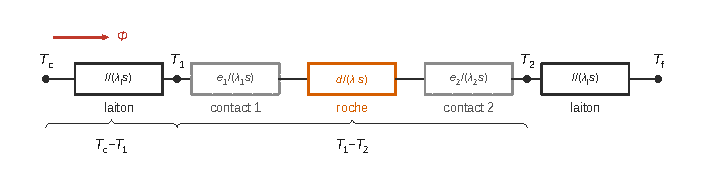
\includegraphics{figures/q21-resistances-serie.pdf}
\caption*{Figure 3 --- schéma équivalent de la figure 5, cinq résistances
thermiques en série traversées par le même flux Φ}
\end{figure}

Le laiton inférieur, puis l'ensemble contact 1, roche et contact 2, donnent :

\equationajustee{\begin{aligned}
T_c-T_1&=\Phi\,\frac{l}{\lambda_l s}\\
T_1-T_2&=\Phi\left(\frac{e_1}{\lambda_1s}+\frac{d}{\lambda s}+\frac{e_2}{\lambda_2s}\right)
\end{aligned}}

Le rapport élimine \(\Phi\) et \(s\) :

\equationajustee{\boxed{\frac{T_1-T_2}{T_c-T_1}=\frac{\lambda_l}{l}\left(\frac{d}{\lambda}+\frac{e_1}{\lambda_1}+\frac{e_2}{\lambda_2}\right)}}

Détermination de \(\lambda\) : le second membre est une fonction affine de \(d\),

\equationajustee{y=\frac{T_1-T_2}{T_c-T_1}=\frac{\lambda_l}{l\lambda}\,d+\frac{\lambda_l}{l}\left(\frac{e_1}{\lambda_1}+\frac{e_2}{\lambda_2}\right)}

On mesure \(y\) pour plusieurs échantillons de la même roche, d'épaisseurs \(d\) différentes, en reproduisant à l'identique les contacts (même serrage, même état de surface). La droite \(y(d)\) a pour pente \(a=\lambda_l/(l\lambda)\), indépendante des contacts, d'où \(\boxed{\lambda=\lambda_l/(l\,a)}\). Les résistances de contact n'affectent que l'ordonnée à l'origine.

\hypertarget{partie-v.2-uxe9volution-de-la-tempuxe9rature-uxe0-lintuxe9rieur-de-la-terre}{%
\subsection{Partie V.2 --- Évolution de la température à l'intérieur de la Terre}\label{partie-v.2-uxe9volution-de-la-tempuxe9rature-uxe0-lintuxe9rieur-de-la-terre}}

\hypertarget{q22}{%
\subsection{Q22}\label{q22}}

\textbf{a)} La sphère homogène de masse \(m\) crée à l'extérieur le champ d'une masse ponctuelle placée en \(O\) (Q2). On adapte donc Q7a, en remplaçant \(M_T\) par \(m\) et \(m\) par \(\mathrm dm\).

Amenée de l'infini à la distance \(r\) de \(O\), la masse \(\mathrm dm\) a l'énergie potentielle :

\equationajustee{\boxed{\mathrm dE_{pG}(r)=-\frac{G\,m\,\mathrm dm}{r}}}

\textbf{b)} Quand la sphère a le rayon \(r\), sa masse est \(m(r)=\frac43\pi r^3\mu\). La coquille suivante apporte \(\mathrm dm=4\pi r^2\mu\,\mathrm dr\) :

\equationajustee{\begin{aligned}
\mathrm dE_{pG}&=-\frac{G}{r}\cdot\frac43\pi r^3\mu\cdot4\pi r^2\mu\,\mathrm dr\\
&=-\frac{16\pi^2}{3}G\mu^2r^4\,\mathrm dr
\end{aligned}}

On intègre de \(r=0\) à \(r=R\) :

\equationajustee{\begin{aligned}
E_{pG}(R)&=-\frac{16\pi^2}{3}G\mu^2\int_0^Rr^4\,\mathrm dr\\
&=-\frac{16\pi^2}{15}G\mu^2R^5
\end{aligned}}

Avec \(\mu=\dfrac{3M}{4\pi R^3}\) :

\equationajustee{\boxed{E_{pG}(R)=-\frac35\,\frac{GM^2}{R}}}

L'énergie est négative : le système est lié ; il faudrait fournir \(\frac35GM^2/R\) pour en disperser la matière à l'infini. Réciproquement, la formation de la sphère a libéré cette énergie.

\hypertarget{q23}{%
\subsection{Q23}\label{q23}}

Toute l'énergie libérée, \(-E_{pG}=\frac35GM_T^2/R_T\), chauffe la Terre de \(0\) K à \(T_{eq}\) :

\equationajustee{\begin{aligned}
M_TC\,T_{eq}&=\frac35\frac{GM_T^2}{R_T}\\
T_{eq}&=\frac{3\,GM_T}{5\,C\,R_T}
\end{aligned}}

\equationajustee{\boxed{T_{eq}=\frac{3\,GM_T}{5\,C\,R_T}}}

Une masse \(M_T\) se simplifie, l'autre subsiste. Contrôle d'homogénéité : \(GM_T/R_T\) s'exprime en \(\mathrm{J\,kg^{-1}}\) et, divisé par \(C\) en \(\mathrm{J\,kg^{-1}\,K^{-1}}\), donne bien une température, positive. Numériquement :

\equationajustee{\begin{aligned}
\log T_{eq}&=\log0{,}6-10{,}17+24{,}78-3{,}00-6{,}81\\
&=-0{,}22+4{,}80\\
&=4{,}58
\end{aligned}}

d'où \(\boxed{T_{eq}\approx4\cdot10^4\ \mathrm K}\).

Cette valeur est très supérieure à la température actuelle du centre de la Terre (de l'ordre de \(6\cdot10^3\) K) : une grande partie de l'énergie d'accrétion a été rayonnée pendant la formation, des changements d'état ont absorbé de l'énergie, et la Terre se refroidit depuis 4,5 milliards d'années. L'énergie d'accrétion suffisait néanmoins largement à fondre la planète.

\hypertarget{q24}{%
\subsection{Q24}\label{q24}}

On sépare les variables : \(\dfrac{\mathrm dN_i}{N_i}=-\dfrac{\ln2}{\tau_i}\mathrm dt\). Avec \(N_i(0)=N_{i0}\) :

\equationajustee{\boxed{\begin{aligned}N_i(t)&=N_{i0}\exp\!\left(-\frac{\ln2}{\tau_i}t\right)\\&=N_{i0}\,2^{-t/\tau_i}\end{aligned}}}

et l'on vérifie \(N_i(\tau_i)=N_{i0}/2\).

\hypertarget{q25}{%
\subsection{Q25}\label{q25}}

\(N_i\) est un nombre de noyaux par unité de volume de roche : c'est une grandeur volumique. Pendant \(\mathrm dt\), le nombre de désintégrations par unité de volume est \(-\mathrm dN_i\), et chacune libère l'énergie \(\varepsilon_i\). La puissance libérée par unité de volume est donc :

\equationajustee{\begin{aligned}
p_{v,i}(t)&=\varepsilon_i\left(-\frac{\mathrm dN_i}{\mathrm dt}\right)\\
&=\varepsilon_i\,\frac{\ln2}{\tau_i}\,N_i(t)
\end{aligned}}

Un volume unité de roche a la masse \(\mu\) et contient la masse \(x_i\mu\) d'isotope. Le nombre initial de noyaux par unité de volume est donc, avec \(M_i\) en \(\mathrm{kg\,mol^{-1}}\) :

\equationajustee{N_{i0}=\frac{x_i\,\mu\,\mathcal N_A}{M_i}}

\equationajustee{\boxed{p_{v,i}(t)=\frac{\ln2\;\varepsilon_i\,x_i\,\mu\,\mathcal N_A}{\tau_i\,M_i}\,e^{-\ln2\,t/\tau_i}}}

Les puissances s'ajoutent, et un même volume de roche contient les trois éléments : la puissance volumique totale est la somme des trois contributions.

\equationajustee{\boxed{p_v(t)=\sum_{i=1}^3\frac{\ln2\;\varepsilon_i\,x_i\,\mu\,\mathcal N_A}{\tau_i\,M_i}\,e^{-\ln2\,t/\tau_i}}}

Contrôle numérique (\(\mu=4{,}5\cdot10^3\ \mathrm{kg\,m^{-3}}\), \(1\ \text{an}=3{,}16\cdot10^7\) s) :

\begin{longtable}[]{@{}
  >{\raggedright\arraybackslash}p{(\columnwidth - 4\tabcolsep) * \real{0.3333}}
  >{\raggedright\arraybackslash}p{(\columnwidth - 4\tabcolsep) * \real{0.3333}}
  >{\raggedright\arraybackslash}p{(\columnwidth - 4\tabcolsep) * \real{0.3333}}@{}}
\toprule\noalign{}
\begin{minipage}[b]{\linewidth}\raggedright
Noyau
\end{minipage} & \begin{minipage}[b]{\linewidth}\raggedright
\(N_{i0}\) (\(\mathrm{m^{-3}}\))
\end{minipage} & \begin{minipage}[b]{\linewidth}\raggedright
\(p_{v,i}(0)\) (\(\mathrm{nW\,m^{-3}}\))
\end{minipage} \\
\midrule\noalign{}
\endhead
\bottomrule\noalign{}
\endlastfoot
\(^{238}\mathrm U\) & \(1{,}5\cdot10^{20}\) & \(5{,}4\) \\
\(^{232}\mathrm{Th}\) & \(4{,}7\cdot10^{20}\) & \(4{,}6\) \\
\(^{40}\mathrm K\) & \(1{,}3\cdot10^{21}\) & \(2{,}6\) \\
\end{longtable}

On obtient \(p_v(0)\approx12{,}5\ \mathrm{nW\,m^{-3}}\), valeur initiale de la figure 6. La puissance totale, grandeur extensive, s'obtient en multipliant par le volume du manteau, \(0{,}84\times\frac43\pi R_T^3=9{,}2\cdot10^{20}\ \mathrm m^3\) : on retrouve \(P\approx1{,}2\cdot10^{13}\) W.

\hypertarget{q26}{%
\subsection{Q26}\label{q26}}

Allure (figure 4) : courbe décroissante et convexe, de \(12{,}5\) à environ \(4\ \mathrm{nW\,m^{-3}}\) en 10 milliards d'années. Ce n'est pas une exponentielle : \(p_v\) est la somme de trois exponentielles de demi-vies différentes (1,26 ; 4,46 ; 14,0 Ga), et sa demi-vie n'est celle d'aucun des trois noyaux.

\begin{figure}[H]
\centering
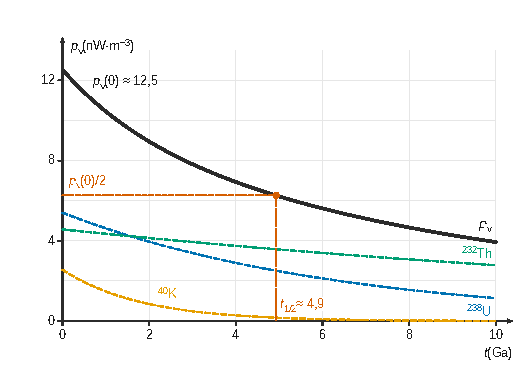
\includegraphics{figures/q26-puissance-radiogenique.pdf}
\caption*{Figure 4 --- p\_v(t) recalculée à partir du tableau 3, ses trois
contributions et la construction de t₁/₂}
\end{figure}

On trace l'horizontale \(p_v=p_v(0)/2\approx6{,}25\ \mathrm{nW\,m^{-3}}\) ; elle coupe la courbe en

\equationajustee{\boxed{t_{1/2}\approx5\cdot10^9\ \text{ans}}\quad(\approx4{,}9\ \text{Ga}).}

Cette durée est comprise entre les demi-vies du potassium et du thorium, proche de celle de l'uranium : le potassium, rapide, s'épuise d'abord, puis la décroissance est dominée par l'uranium et le thorium.

\hypertarget{q27}{%
\subsection{Q27}\label{q27}}

La « source » de la diffusion thermique est l'inhomogénéité de température : d'après la loi de Fourier, \(\vec j=-\lambda\,\overrightarrow{\mathrm{grad}}\,T\). On étudie donc les causes qui fixent le champ de température :

\begin{itemize}
\tightlist
\item
  le milieu, homogène (\(\mu\), \(C\) et \(\lambda\) uniformes) ;
\item
  les sources radioactives, réparties avec la symétrie sphérique ;
\item
  la condition aux limites, une température de surface uniforme.
\end{itemize}

Ces causes sont invariantes par toute rotation autour de \(O\). Le champ de température l'est aussi : \(T\) ne dépend ni de \(\theta\) ni de \(\varphi\), mais seulement de \(r\) et de \(t\).

\equationajustee{T(M,t)=T(r,t)}

Avec l'expression du gradient rappelée par l'énoncé :

\equationajustee{\begin{aligned}
\vec j&=-\lambda\,\overrightarrow{\mathrm{grad}}\,T\\
&=-\lambda\,\frac{\partial T}{\partial r}\,\vec u_r
\end{aligned}}

\equationajustee{\boxed{\begin{aligned}\vec j&=j(r,t)\,\vec u_r\\j(r,t)&=-\lambda\,\frac{\partial T}{\partial r}\end{aligned}}}

Invariances : par toute rotation autour de \(O\), donc aucune dépendance en \(\theta\) ni en \(\varphi\) ; \(j\) ne dépend que de \(r\) et de \(t\).

\hypertarget{q28}{%
\subsection{Q28}\label{q28}}

Système : la coquille comprise entre \(r\) et \(r+\mathrm dr\), de volume \(4\pi r^2\mathrm dr\), solide indéformable et immobile. Premier principe entre \(t\) et \(t+\mathrm dt\) : \(\mathrm dU=\delta Q\), aucun travail n'étant échangé.

\begin{itemize}
\tightlist
\item
  \(\mathrm dU=\mu\,4\pi r^2\mathrm dr\,C\,\dfrac{\partial T}{\partial t}\mathrm dt\) : \textbf{variation d'énergie interne} de la coquille.
\item
  Elle reçoit par conduction \(\Phi(r)\,\mathrm dt\) par sa face interne et cède \(\Phi(r+\mathrm dr)\,\mathrm dt\) par sa face externe, avec \(\Phi=j\,4\pi r^2\).
\item
  Le transfert net est donc \(\delta Q_{\rm cond}=-\mathrm d\!\left(j\,4\pi r^2\right)\mathrm dt\) : \textbf{bilan net des échanges conductifs} (énergie entrante moins sortante).
\item
  La radioactivité y produit \(\delta Q_{\rm prod}=p'_v\,4\pi r^2\mathrm dr\,\mathrm dt\) : \textbf{énergie produite dans le volume} par les sources internes.
\end{itemize}

\equationajustee{\boxed{\mu C\,4\pi r^2\frac{\partial T}{\partial t}\,\mathrm dt\,\mathrm dr=-\mathrm d\!\left(j\,4\pi r^2\right)\mathrm dt+p'_v\,4\pi r^2\,\mathrm dr\,\mathrm dt}}

\hypertarget{q29}{%
\subsection{Q29}\label{q29}}

\textbf{a)} En régime stationnaire, le premier membre de Q28 est nul ; on divise par \(4\pi\,\mathrm dr\,\mathrm dt\) :

\equationajustee{\frac{\mathrm d}{\mathrm dr}\left(r^2j\right)=p'_v\,r^2}

Avec \(j=-\lambda\,\dfrac{\mathrm dT}{\mathrm dr}\) :

\equationajustee{\boxed{\frac1{r^2}\frac{\mathrm d}{\mathrm dr}\left(r^2\frac{\mathrm dT}{\mathrm dr}\right)=-\frac{p'_v}{\lambda}}}

\textbf{b)} On intègre l'équation sous cette forme, sans développer la dérivée. Avec \(p'_v\) uniforme et deux constantes \(A\) et \(B\) :

\equationajustee{\begin{aligned}
r^2\frac{\mathrm dT}{\mathrm dr}&=-\frac{p'_v}{3\lambda}r^3+A\\
T(r)&=-\frac{p'_v}{6\lambda}r^2-\frac Ar+B
\end{aligned}}

\(T\) finie en \(r=0\) impose \(A=0\), et \(T(R_T)=T_s\) donne \(B\) :

\equationajustee{\boxed{T(r)=T_s+\frac{p'_v}{6\lambda}\left(R_T^2-r^2\right)}}

Le profil est parabolique, maximal au centre.

\textbf{c)}

\equationajustee{\boxed{\begin{aligned}j(r)&=-\lambda\frac{\mathrm dT}{\mathrm dr}\\&=\frac{p'_v\,r}{3}\end{aligned}}}

(Contrôle : \(4\pi r^2j(r)=\frac43\pi r^3p'_v\), puissance produite dans la boule de rayon \(r\).)

\textbf{d)} En \(r=R_T\) :

\equationajustee{\begin{aligned}
p'_v&=\frac{3\,j(R_T)}{R_T}\\
&=\frac{3\times70\cdot10^{-3}}{6{,}4\cdot10^6}\\
&\approx\boxed{3\cdot10^{-8}\ \mathrm{W\,m^{-3}}}
\end{aligned}}

soit environ \(33\ \mathrm{nW\,m^{-3}}\).

D'après Q25--Q26, la radioactivité fournit actuellement \(p_v\approx12{,}5\ \mathrm{nW\,m^{-3}}\), soit environ trois fois moins, et encore moins rapporté à toute la Terre, puisqu'elle n'est attribuée qu'au manteau.

La radioactivité n'explique donc qu'une partie (de l'ordre de 40 \%) du flux géothermique. Le reste est de la chaleur héritée de la formation (Q23) que la Terre évacue en se refroidissant : l'hypothèse de régime stationnaire n'est pas justifiée.

Par ailleurs, avec \(\lambda\approx3\ \mathrm{W\,K^{-1}\,m^{-1}}\), le profil de (b) donnerait au centre \(T(0)\approx7\cdot10^4\) K, valeur irréaliste. La chaleur est en réalité évacuée surtout par convection dans le manteau, bien plus efficace que la conduction.

\hypertarget{partie-vi-le-champ-magnuxe9tique-terrestre}{%
\section{Partie VI --- Le champ magnétique terrestre}\label{partie-vi-le-champ-magnuxe9tique-terrestre}}

\hypertarget{q30}{%
\subsection{Q30}\label{q30}}

On projette \(\vec u_z\) sur la base sphérique par produits scalaires : \(\vec u_z\cdot\vec u_r=\cos\theta\), \(\vec u_z\cdot\vec u_\theta=-\sin\theta\) et \(\vec u_z\cdot\vec u_\varphi=0\). Donc :

\equationajustee{\begin{aligned}
\vec u_z&=\cos\theta\,\vec u_r-\sin\theta\,\vec u_\theta\\
\vec m&=-m\cos\theta\,\vec u_r+m\sin\theta\,\vec u_\theta\\
\vec m\cdot\vec r&=-mr\cos\theta
\end{aligned}}

En reportant dans l'expression intrinsèque, avec \(\vec r=r\,\vec u_r\) :

\equationajustee{\vec B=\frac{\mu_0}{4\pi r^3}\left[-3m\cos\theta\,\vec u_r+m\cos\theta\,\vec u_r-m\sin\theta\,\vec u_\theta\right]}

\equationajustee{\boxed{\begin{aligned}B_r&=-\frac{\mu_0m\cos\theta}{2\pi r^3}\\B_\theta&=-\frac{\mu_0m\sin\theta}{4\pi r^3}\\B_\varphi&=0\end{aligned}}}

(\(B_\varphi=0\) : tout plan méridien est plan d'antisymétrie de la distribution de courants équivalente, le champ y est contenu.)

\hypertarget{q31}{%
\subsection{Q31}\label{q31}}

Une ligne de champ est une courbe tangente en chacun de ses points au champ \(\vec B\). Le déplacement élémentaire le long de la ligne vérifie donc \(\mathrm d\vec\ell\wedge\vec B=\vec 0\).

Dans un plan méridien (\(B_\varphi=0\)), \(\mathrm d\vec\ell=\mathrm dr\,\vec u_r+r\,\mathrm d\theta\,\vec u_\theta\) est colinéaire à \(\vec B\). Pour \(0<\theta<\pi\) :

\equationajustee{\begin{aligned}
\frac{\mathrm dr}{B_r}&=\frac{r\,\mathrm d\theta}{B_\theta}\\
\frac{\mathrm dr}{r}&=\frac{2\cos\theta}{\sin\theta}\,\mathrm d\theta
\end{aligned}}

d'où \(\ln r=2\ln\sin\theta+\text{cte}\) :

\equationajustee{\boxed{r(\theta)=K\sin^2\theta,\qquad K>0}}

Allure (figure 5) : chaque ligne est une boucle qui part de \(O\) et y revient (\(r\to0\) aux pôles). Elle coupe le plan équatorial en \(r=K\) ; les boucles sont symétriques par rapport à ce plan et emboîtées, et l'axe des pôles est lui-même une ligne de champ.

\begin{figure}[H]
\centering
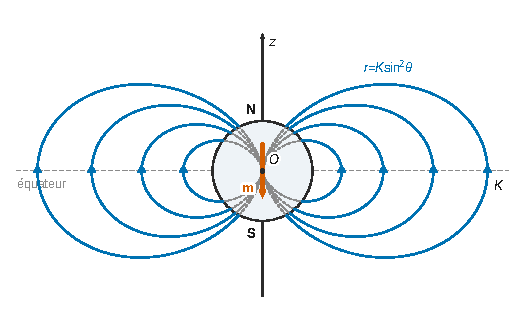
\includegraphics{figures/q31-lignes-champ-dipole.pdf}
\caption*{Figure 5 --- lignes de champ r = K sin²θ du dipôle terrestre dans un
plan méridien, orientées du sud vers le nord à l'extérieur}
\end{figure}

Sens : au pôle Nord (\(\theta=0\)), \(B_r<0\) ; à l'équateur, \(B_\theta<0\), champ dirigé vers le nord. À l'extérieur de la Terre, \textbf{les lignes de champ vont du pôle Sud géographique vers le pôle Nord géographique}, où elles rentrent dans le sol.

\hypertarget{q32}{%
\subsection{Q32}\label{q32}}

À la surface (\(r=R_T\)), \(\vec u_r\) est la verticale ascendante et \(\vec u_\theta\) l'horizontale du méridien dirigée vers le sud.

Avec \(\Lambda=\pi/2-\theta\), on a \(\cos\theta=\sin\Lambda\) et \(\sin\theta=\cos\Lambda\) :

\equationajustee{\boxed{\begin{aligned}B_h&=|B_\theta|=\frac{\mu_0m\cos\Lambda}{4\pi R_T^3}\quad\text{(\text{dirigée} vers le nord)}\\B_v&=B_r=-\frac{\mu_0m\sin\Lambda}{2\pi R_T^3}\end{aligned}}}

\(B_v\) est compté sur la verticale ascendante : dans l'hémisphère Nord, le champ plonge vers le sol. On a \(|B_v|/B_h=2\tan\Lambda\) : le champ est horizontal à l'équateur et vertical aux pôles.

\hypertarget{q33}{%
\subsection{Q33}\label{q33}}

À l'équateur (\(\Lambda=0\)), \(B_v=0\) et \(B=B_h=\dfrac{\mu_0m}{4\pi R_T^3}\), d'où, avec \(\mu_0/4\pi=10^{-7}\ \mathrm{H\,m^{-1}}\) :

\equationajustee{\boxed{\begin{aligned}m&=\frac{4\pi R_T^3B}{\mu_0}\\&=\frac{R_T^3B}{10^{-7}}\end{aligned}}}

\equationajustee{\begin{aligned}
\log m&=3\times6{,}81+\log(2{,}6\cdot10^{-5})+7\\
&=20{,}43-4{,}59+7\\
&=22{,}84
\end{aligned}}

d'où \(\boxed{m\approx7\cdot10^{22}\ \mathrm{A\,m^2}}\).

FIN

\end{document}
